\chapter{幂级数}

\section{幂 级 数}

本章将讨论由幂函数序列 \(\left\{  {{a}_{n}{\left( x - {x}_{0}\right) }^{n}}\right\}\) 所产生的函数项级数
\[
\mathop{\sum }\limits_{{n = 0}}^{\infty }{a}_{n}{\left( x - {x}_{0}\right) }^{n} = {a}_{0} + {a}_{1}\left( {x - {x}_{0}}\right)  + {a}_{2}{\left( x - {x}_{0}\right) }^{2} + \cdots  + {a}_{n}{\left( x - {x}_{0}\right) }^{n} + \cdots , \tag{1}
\]
它称为幂级数, 是一类最简单的函数项级数, 从某种意义上说, 它也可以看作是多项式函数的延伸. 幂级数在理论和实际上都有很多应用, 特别在应用它表示函数方面, 使我们对它的作用有许多新的认识.

下面将着重讨论 \({x}_{0} = 0\) ,即
\[
\mathop{\sum }\limits_{{n = 0}}^{\infty }{a}_{n}{x}^{n} = {a}_{0} + {a}_{1}x + {a}_{2}{x}^{2} + \cdots  + {a}_{n}{x}^{n} + \cdots  \tag{2}
\]
的情形,因为只要把 (2) 中的 \(x\) 换成 \(x - {x}_{0}\) ,就得到 (1).

\subsection{幂级数的收敛区间}

首先讨论幂级数 (2) 的收敛性问题. 显然任意一个幂级数 (2) 在 \(x = 0\) 处总是收敛的. 除此之外, 它还在哪些点收敛? 我们有下面重要的定理.

%定理 14.1
\begin{theorem}{}{the:}

\end{theorem}
 (阿贝尔定理) 若幂级数 (2) 在 \(x = \bar{x} \neq  0\) 处收敛,则对满足不等式 \(\left| x\right|\)  \(< \left| \bar{x}\right|\) 的任何 \(x\) ,幂级数 (2) 收敛而且绝对收敛; 若幂级数 (2) 在 \(x = \bar{x}\) 处发散,则对满足不等式 \(\left| x\right|  > \left| \bar{x}\right|\) 的任何 \(x\) ,幂级数 (2) 发散.

%证
\begin{proof}

\end{proof}
设级数 \(\mathop{\sum }\limits_{{n = 0}}^{\infty }{a}_{n}{\bar{x}}^{n}\) 收敛,从而数列 \(\left\{  {{a}_{n}{\bar{x}}^{n}}\right\}\) 收敛于零且有界,即存在某正数 \(M\) ,使得
\[
\left| {{a}_{n}{\bar{x}}^{n}}\right|  < M\;\left( {n = 0,1,2,\cdots }\right) .
\]
另一方面,对任意一个满足不等式 \(\left| x\right|  < \left| \bar{x}\right|\) 的 \(x\) ,设
\[
r = \left| \frac{x}{\bar{x}}\right|  < 1,
\]
则有
\[
\left| {{a}_{n}{x}^{n}}\right|  = \left| {{a}_{n}{\bar{x}}^{n} \cdot  \frac{{x}^{n}}{{\bar{x}}^{n}}}\right|  = \left| {{a}_{n}{\bar{x}}^{n}}\right|  \cdot  {\left| \frac{x}{\bar{x}}\right| }^{n} < M{r}^{n}.
\]
由于级数 \(\mathop{\sum }\limits_{{n = 0}}^{\infty }M{r}^{n}\) 收敛,故幂级数 (2) 当 \(\left| x\right|  < \left| \bar{x}\right|\) 时绝对收敛.

现在证明定理的第二部分. 设幂级数 (2) 在 \(x = \bar{x}\) 处发散,如果存在某一个 \({x}_{0}\) ,它满足不等式 \(\left| {x}_{0}\right|  > \left| \bar{x}\right|\) ,且使级数 \(\mathop{\sum }\limits_{{n = 0}}^{\infty }{a}_{n}{x}_{0}^{n}\) 收敛. 则由定理第一部分知道,幂级数 (2) 应在 \(x = \bar{x}\) 处绝对收敛,这与假设相矛盾,所以对一切满足不等式 \(\left| x\right|  > \left| \bar{x}\right|\) 的 \(x\) ,幂级数 ( 2 ) 都发散.

由此定理知道: 幂级数 (2) 的收敛域是以原点为中心的区间. 若以 \({2R}\) 表示区间的长度,则称 \(R\) 为幂级数的收敛半径. 实际上,它就是使得幂级数 (2) 收敛的那些收敛点的绝对值的上确界. 所以

当 \(R = 0\) 时,幂级数 (2) 仅在 \(x = 0\) 处收敛;

当 \(R =  + \infty\) 时,幂级数 (2) 在 \(\left( {-\infty , + \infty }\right)\) 上收敛;

当 \(0 < R <  + \infty\) 时,幂级数 (2) 在(-R, R)上收敛; 对一切满足不等式 \(\left| x\right|  > R\) 的 \(x\) ,幂级数 (2) 都发散; 至于在 \(x =  \pm  R\) 处,则幂级数 (2) 可能收敛也可能发散.

我们称(-R, R)为幂级数 (2) 的收敛区间.

怎样求得幂级数 (2) 的收敛半径, 有如下定理.

%定理 14.2
\begin{theorem}{}{the:}

\end{theorem}
 对于幂级数 (2) , 若
\[
\mathop{\lim }\limits_{{n \rightarrow  \infty }}\sqrt[n]{\left| {a}_{n}\right| } = \rho , \tag{3}
\]
则当

(i) \(0 < \rho  <  + \infty\) 时,幂级数 (2) 的收敛半径 \(R = \frac{1}{\rho }\) ;

(ii) \(\rho  = 0\) 时,幂级数 (2) 的收敛半径 \(R =  + \infty\) ;

(iii) \(\rho  =  + \infty\) 时,幂级数 (2) 的收敛半径 \(R = 0\) .

%证
\begin{proof}

\end{proof}
对于幂级数 \(\mathop{\sum }\limits_{{n = 0}}^{\infty }\left| {{a}_{n}{x}^{n}}\right|\) ,由于
\[
\mathop{\lim }\limits_{{n \rightarrow  \infty }}\sqrt[n]{\left| {a}_{n}{x}^{n}\right| } = \mathop{\lim }\limits_{{n \rightarrow  \infty }}\sqrt[n]{\left| {a}_{n}\right| }\left| x\right|  = \rho \left| x\right| ,
\]
根据级数的根式判别法,当 \(\rho \left| x\right|  < 1\) 时, \(\mathop{\sum }\limits_{{n = 0}}^{\infty }\left| {{a}_{n}{x}^{n}}\right|\) 收敛; 当 \(\rho \left| x\right|  > 1\) 时, \(\mathop{\sum }\limits_{{n = 0}}^{\infty }\left| {{a}_{n}{x}^{n}}\right|\) 发散. 于是当 \(0 < \rho  <  + \infty\) 时,由 \(\rho \left| x\right|  < 1\) 得幂级数 (2) 的收敛半径 \(R = \frac{1}{\rho }\) . 当 \(\rho  = 0\) 时, 对任何 \(x\) 皆有 \(\rho \left| x\right|  < 1\) ,所以 \(R =  + \infty\) . 当 \(\rho  =  + \infty\) 时,则对除 \(x = 0\) 外的任何 \(x\) 皆有 \(\rho \left| x\right|  > 1\) ,所以 \(R = 0\) .

在第十二章 §2 第二段曾经指出: 若 \(\mathop{\lim }\limits_{{n \rightarrow  \infty }}\frac{\left| {a}_{n + 1}\right| }{\left| {a}_{n}\right| } = \rho\) ,则有 \(\mathop{\lim }\limits_{{n \rightarrow  \infty }}\sqrt[n]{\left| {a}_{n}\right| } = \rho\) . 因此,我们也常用级数的比式判别法来推出幂级数 (2) 的收敛半径.

%例 1
\begin{example}

\end{example}
考察级数 \(\mathop{\sum }\limits_{{n = 1}}^{\infty }\frac{{x}^{n}}{{n}^{2}}\) ,由于
\[
\frac{{a}_{n + 1}}{{a}_{n}} = \frac{{n}^{2}}{{\left( n + 1\right) }^{2}} \rightarrow  1\left( {n \rightarrow  \infty }\right) ,
\]
所以它的收敛半径 \(R = 1\) ,即收敛区间为(-1,1); 当 \(x =  \pm  1\) 时,有 \(\left| \frac{{\left( \pm 1\right) }^{n}}{{n}^{2}}\right|  = \frac{1}{{n}^{2}}\) ,由于级数 \(\mathop{\sum }\limits_{{n = 1}}^{\infty }\frac{1}{{n}^{2}}\) 收敛,所以级数 \(\mathop{\sum }\limits_{{n = 1}}^{\infty }\frac{{x}^{n}}{{n}^{2}}\) 在 \(x =  \pm  1\) 时也收敛. 于是这个级数的收敛域为 \(\left\lbrack  {-1,1}\right\rbrack\) .

%例 2
\begin{example}

\end{example}
考察级数
\[
x + \frac{{x}^{2}}{2} + \cdots  + \frac{{x}^{n}}{n} + \cdots , \tag{4}
\]
由于
\[
R = \mathop{\lim }\limits_{{n \rightarrow  \infty }}\frac{{a}_{n}}{{a}_{n + 1}} = \mathop{\lim }\limits_{{n \rightarrow  \infty }}\frac{n + 1}{n} = 1,
\]
所以幂级数 (4) 的收敛区间是(-1,1). 但级数 (4) 当 \(x = 1\) 时发散, \(x =  - 1\) 时收敛,从而推得级数 (4) 的收敛域是半开区间 \(\lbrack  - 1,1)\) .

照此方法, 读者不难验证级数
\[
\mathop{\sum }\limits_{{n = 0}}^{\infty }\frac{{x}^{n}}{n!}\text{ 与 }\mathop{\sum }\limits_{{n = 0}}^{\infty }n!{x}^{n}
\]
的收敛半径分别为 \(R =  + \infty\) 与 \(R = 0\) .

%定理 14.3
\begin{theorem}{}{the:}

\end{theorem}
(柯西-阿达马(Cauchy-Hadamard)定理)对于幂级数(2),设
\[
\rho  = \mathop{\lim }\limits_{{n \rightarrow  \infty }}\sqrt[n]{\left| {a}_{n}\right| }, \tag{5}
\]
则当

(i) \(0 < \rho  <  + \infty\) 时,收敛半径 \(R = \frac{1}{\rho }\) ;

(ii) \(\rho  = 0\) 时, \(R =  + \infty\) ;

(iii) \(\rho  =  + \infty\) 时, \(R = 0\) .

注意: 由于上极限 (5) 总是存在的, 因而任一幂级数总能由 (5) 式得到它的收敛半径.

%定理 14.3
\begin{theorem}{}{the:}

\end{theorem}
 的证明与定理 14.2 相仿, 读者可自行根据定理 12.8 推论 2 推出.

%例 3
\begin{example}

\end{example}
考察级数
\[
1 + \frac{x}{3} + \frac{{x}^{2}}{{2}^{2}} + \frac{{x}^{3}}{{3}^{3}} + \frac{{x}^{4}}{{2}^{4}} + \cdots  + \frac{{x}^{{2n} - 1}}{{3}^{{2n} - 1}} + \frac{{x}^{2n}}{{2}^{2n}} + \cdots ,
\]
由于
\[
\mathop{\lim }\limits_{{n \rightarrow  \infty }}\sqrt[n]{{a}_{n}} = \frac{1}{2},
\]
所以收敛半径 \(R = 2\) . 由于 \(x =  \pm  2\) 时,这两个数项级数都发散. 故级数的收敛域为(-2,2).

%例 4
\begin{example}

\end{example}
求 \(\mathop{\sum }\limits_{{n = 1}}^{\infty }\frac{{x}^{2n}}{n - {3}^{2n}}\) 的收敛域.

%解
\begin{solution}

\end{solution}
这是一个缺项幂级数, 可以用定理 14.3 求收敛半径, 也可以用下面的方法来求.

因为当 \(\mathop{\lim }\limits_{{n \rightarrow  \infty }}\sqrt[n]{\frac{{x}^{2n}}{\left| n - {3}^{2n}\right| }} = \frac{1}{9}\mathop{\lim }\limits_{{n \rightarrow  \infty }}\sqrt[n]{\frac{{x}^{2n}}{1 - \frac{n}{{3}^{2n}}}} = \frac{{x}^{2}}{9} < 1\) ,即 \(\left| x\right|  < 3\) 时级数收敛,所以原级数的收敛半径为 \(R = 3\) . 又当 \(x =  \pm  3\) 时,相应的级数都是 \(\mathop{\sum }\limits_{{n = 1}}^{\infty }\frac{{3}^{2n}}{n - {3}^{2n}}\) ,而 \(\mathop{\lim }\limits_{{n \rightarrow  \infty }}\frac{{3}^{2n}}{n - {3}^{2n}} =  - 1 \neq  0\) ,

级数 \(\mathop{\sum }\limits_{{n = 1}}^{\infty }\frac{{3}^{2n}}{n - {3}^{2n}}\) 发散. 因此原级数的收敛域为(-3,3).

下面讨论幂级数 (2) 的一致收敛性问题.

%定理 14.4
\begin{theorem}{}{the:}

\end{theorem}
 若幂级数 (2) 的收敛半径为 \(R\left( { > 0}\right)\) ,则幂级数 (2) 在它的收敛区间 (-R, R)内任一闭区间 \(\left\lbrack  {a,b}\right\rbrack\) 上都一致收敛.

%证
\begin{proof}

\end{proof}
设 \(\bar{x} = \max \{ \left| a\right| ,\left| b\right| \}  \in  \left( {-R,R}\right)\) ,那么对于 \(\left\lbrack  {a,b}\right\rbrack\) 上任一点 \(x\) ,都有
\[
\left| {{a}_{n}{x}^{n}}\right|  \leq  \left| {{a}_{n}{\bar{x}}^{n}}\right| .
\]
由于级数 (2) 在点 \(\bar{x}\) 绝对收敛,应用优级数判别法推得级数 (2) 在 \(\left\lbrack  {a,b}\right\rbrack\) 上一致收敛.

%定理 14.5
\begin{theorem}{}{the:}

\end{theorem}
 若幂级数 (2) 的收敛半径为 \(R\left( { > 0}\right)\) ,且在 \(x = R\) (或 \(x =  - R\) ) 时收敛, 则级数 (2) 在 \(\left\lbrack  {0,R}\right\rbrack\) (或 \(\left\lbrack  {-R,0}\right\rbrack\) ) 上一致收敛.

%证
\begin{proof}

\end{proof}
设级数 (2) 在 \(x = R\) 时收敛,对于 \(x \in  \left\lbrack  {0,R}\right\rbrack\) 有
\[
\mathop{\sum }\limits_{{n = 0}}^{\infty }{a}_{n}{x}^{n} = \mathop{\sum }\limits_{{n = 0}}^{\infty }{a}_{n}{R}^{n}{\left( \frac{x}{R}\right) }^{n}.
\]
已知级数 \(\mathop{\sum }\limits_{{n = 0}}^{\infty }{a}_{n}{R}^{n}\) 收敛,函数列 \(\left\{  {\left( \frac{x}{R}\right) }^{n}\right\}\) 在 \(\left\lbrack  {0,R}\right\rbrack\) 上递减且一致有界,即
\[
1 \geq  \frac{x}{R} \geq  {\left( \frac{x}{R}\right) }^{2} \geq  \cdots  \geq  {\left( \frac{x}{R}\right) }^{n} \geq  \cdots  \geq  0.
\]
故由阿贝尔判别法 (定理 13.6 ),级数 (2) 在 \(\left\lbrack  {0,R}\right\rbrack\) 上一致收敛.

关于一般幂级数 (1) 的收敛性问题, 也可仿照上述的办法来确定它的收敛区间和收敛半径.

%例 5
\begin{example}

\end{example}
考察级数
\[
\mathop{\sum }\limits_{{n = 1}}^{\infty }\frac{{\left( x - 1\right) }^{n}}{{2}^{n}n} = \frac{x - 1}{2} + \frac{{\left( x - 1\right) }^{2}}{{2}^{2} \cdot  2} + \cdots  + \frac{{\left( x - 1\right) }^{n}}{{2}^{n} \cdot  n} + \cdots , \tag{6}
\]
由于
\[
\frac{\frac{1}{{2}^{n + 1}\left( {n + 1}\right) }}{\frac{1}{{2}^{n} \cdot  n}} = \frac{n}{2\left( {n + 1}\right) } \rightarrow  \frac{1}{2}\;\left( {n \rightarrow  \infty }\right) ,
\]
因此级数 (6) 的收敛半径 \(R = 2\) ,因而它的收敛区间为 \(\left| {x - 1}\right|  < 2\) ,即(-1,3). 当 \(x =  - 1\) 时, 级数 (6) 为收敛级数
\[
\mathop{\sum }\limits_{{n = 1}}^{\infty }\frac{{\left( -2\right) }^{n}}{{2}^{n} \cdot  n} =  - 1 + \frac{1}{2} - \frac{1}{3} + \cdots  + {\left( -1\right) }^{n}\frac{1}{n} + \cdots ;
\]
当 \(x = 3\) 时,级数 (6) 为发散级数
\[
\mathop{\sum }\limits_{{n = 1}}^{\infty }\frac{{2}^{n}}{{2}^{n}n} = \sum \frac{1}{n} = 1 + \frac{1}{2} + \frac{1}{3} + \cdots  + \frac{1}{n} + \cdots .
\]
于是级数 (6) 的收敛域为 \(\lbrack  - 1,3)\) .

\subsection{幂级数的性质}

首先由定理 13.12 立刻可得

%定理 14.6
\begin{theorem}{}{the:}

\end{theorem}
 (i) 幂级数 (2) 的和函数是(-R, R)上的连续函数; (ii) 若幂级数 (2) 在收敛区间的左 (右) 端点上收敛, 则其和函数也在这一端点上右 (左) 连续.

在讨论幂级数的逐项求导与逐项求积之前, 先要确定幂级数 (2) 在收敛区间 (-R, R)上逐项求导与逐项求积后所得到的幂级数
\[
{a}_{1} + 2{a}_{2}x + 3{a}_{3}{x}^{2} + \cdots  + n{a}_{n}{x}^{n - 1} + \cdots  \tag{7}
\]
与
\[
{a}_{0}x + \frac{{a}_{1}}{2}{x}^{2} + \frac{{a}_{2}}{3}{x}^{3} + \cdots  + \frac{{a}_{n}}{n + 1}{x}^{n + 1} + \cdots  \tag{8}
\]
的收敛区间.

%定理 14.7
\begin{theorem}{}{the:}

\end{theorem}
 幂级数 (2) 与幂级数 (7)、(8) 具有相同的收敛区间.

%证
\begin{proof}

\end{proof}
这里只要证明 (2) 与 (7) 具有相同的收敛区间就可以了, 因为对 (8) 逐项求导就得到(2).

设 \({x}_{0}\) 为幂级数 (2) 在其收敛区间(-R, R)内任一不为零的点. 由阿贝尔定理 (定理 14.1) 的证明知道,存在正数 \(M\) 与 \(r\left( {r < 1}\right)\) ,对一切正整数 \(n\) ,都有
\[
\left| {{a}_{n}{x}_{0}^{n}}\right|  < M{r}^{n}.
\]
于是
\[
\left| {n{a}_{n}{x}_{0}^{n - 1}}\right|  = \left| \frac{n}{{x}_{0}}\right| \left| {{a}_{n}{x}_{0}^{n}}\right|  < \frac{M}{\left| {x}_{0}\right| }n{r}^{n},
\]
由级数的比式判别法知道,级数 \(\mathop{\sum }\limits_{{n = 0}}^{\infty }n{r}^{n}\) 收敛. 根据级数的比较原则及上述不等式,推知幂级数 (7) 在点 \({x}_{0}\) 是绝对收敛的 (当然也是收敛的! ). 由于 \({x}_{0}\) 为(-R, R)上任一点, 这就证得幂级数 (7) 在(-R, R)上收敛.

现在证明幂级数 (7) 对一切满足不等式 \(\left| x\right|  > R\) 的 \(x\) 都不收敛. 如若不然,幂级数 (7) 在点 \({x}_{0}\left( {\left| {x}_{0}\right|  > R}\right)\) 收敛,则有一数 \(\bar{x}\) ,使得 \(\left| {x}_{0}\right|  > \left| \bar{x}\right|  > R\) . 由阿贝尔定理,幂级数 (7) 在 \(x = \bar{x}\) 处绝对收敛. 但是,取 \(n \geq  \left| \bar{x}\right|\) 时,就有
\[
\left| {n{a}_{n}{\bar{x}}^{n - 1}}\right|  = \frac{n}{\left| \bar{x}\right| }\left| {{a}_{n}{\bar{x}}^{n}}\right|  \geq  \left| {{a}_{n}{\bar{x}}^{n}}\right| ,
\]
由比较原则得幂级数 (2) 在 \(x = \bar{x}\) 处绝对收敛. 这与所设幂级数 (2) 的收敛区间为 (-R, R)相矛盾. 这就证明了幂级数 (7) 的收敛区间也是(-R, R).

%定理 14.8
\begin{theorem}{}{the:}

\end{theorem}
 设幂级数 (2) 在收敛区间(-R, R)上的和函数为 \(f\) ,若 \(x\) 为(-R, R)上任意一点, 则

(i) \(f\) 在点 \(x\) 可导,且
\[
{f}^{\prime }\left( x\right)  = \mathop{\sum }\limits_{{n = 1}}^{\infty }n{a}_{n}{x}^{n - 1};
\]
(ii) \(f\) 在 0 与 \(x\) 之间的这个区间上可积,且
\[
{\int }_{0}^{x}f\left( t\right) \mathrm{d}t = \mathop{\sum }\limits_{{n = 0}}^{\infty }\frac{{a}_{n}}{n + 1}{x}^{n + 1}.
\]
%定理 14.8
\begin{theorem}{}{the:}

\end{theorem}
 指出幂级数在收敛区间内可逐项求导与逐项求积.

%证
\begin{proof}

\end{proof}
由定理 14.7 知,级数 \(\left( 2\right) ,\left( 7\right) ,\left( 8\right)\) 具有相同的收敛半径 \(R\) . 因此,对任意一点 \(x \in  \left( {-R,R}\right)\) ,总存在正数 \(r\) ,使得 \(\left| x\right|  < r < R\) ,根据定理 14.4,级数 (2),(7) 在 \(\left\lbrack  {-r,r}\right\rbrack\) 上一致收敛. 再由第十三章 §2 的逐项求导与逐项求积定理, 就得到所要证明的结论 (i) 与 (ii).

由定理 14.8 的 (i) 可得:

推论 1 记 \(f\) 为幂级数 (2) 在收敛区间(-R, R)上的和函数,则在(-R, R)上 \(f\) 具有任何阶导数, 且可逐项求导任何次, 即
\[
{f}^{\prime }\left( x\right)  = {a}_{1} + 2{a}_{2}x + 3{a}_{3}{x}^{2} + \cdots  + n{a}_{n}{x}^{n - 1} + \cdots ,
\]
\[
{f}^{\prime \prime }\left( x\right)  = 2{a}_{2} + 3 \cdot  2{a}_{3}x + \cdots  + n\left( {n - 1}\right) {a}_{n}{x}^{n - 2} + \cdots ,
\]
............
\[
{f}^{\left( n\right) }\left( x\right)  = n!{a}_{n} + \left( {n + 1}\right) n\left( {n - 1}\right) \cdots 2{a}_{n + 1}x + \cdots ,
\]
............

推论 2 记 \(f\) 为幂级数 (2) 在点 \(x = 0\) 某邻域上的和函数,则幂级数 (2) 的系数与 \(f\) 在 \(x = 0\) 处的各阶导数有如下关系:
\[
{a}_{0} = f\left( 0\right) ,\;{a}_{n} = \frac{{f}^{\left( n\right) }\left( 0\right) }{n!}\left( {n = 1,2,\cdots }\right) .
\]
这个推论还表明,若幂级数 (2) 在(-R, R)上有和函数 \(f\) ,则幂级数 (2) 由 \(f\) 在点 \(x = 0\) 处的各阶导数所惟一确定.

\subsection{幂级数的运算}

在讨论幂级数的运算之前, 先说明两个幂级数

与
\[
\mathop{\sum }\limits_{{n = 0}}^{\infty }{a}_{n}{x}^{n} = {a}_{0} + {a}_{1}x + \cdots  + {a}_{n}{x}^{n} + \cdots  \tag{2}
\]
\[
\mathop{\sum }\limits_{{n = 0}}^{\infty }{b}_{n}{x}^{n} = {b}_{0} + {b}_{1}x + \cdots  + {b}_{n}{x}^{n} + \cdots  \tag{9}
\]
相等的意义.

%定义  1
\begin{definition}{}{def:}

\end{definition}
若幂级数 (2) 与 (9) 在点 \(x = 0\) 的某邻域内有相同的和函数,则称这两个幂级数在该邻域内相等.

%定理 14.9
\begin{theorem}{}{the:}

\end{theorem}
 若幂级数 (2) 与 (9) 在点 \(x = 0\) 的某邻域内相等,则它们同次幂项的系数相等, 即
\[
{a}_{n} = {b}_{n}\;\left( {n = 0,1,2,\cdots }\right) .
\]
这个定理的结论可直接由定理 14.8 的推论 2 得到.

根据这个定理还可推得:若幂级数 (2) 的和函数为奇 (偶) 函数, 则 (2) 式不出现偶 (奇)次幂的项.

%定理 14.10
\begin{theorem}{}{the:}

\end{theorem}
 若幂级数 (2) 与 (9) 的收敛半径分别为 \({R}_{a}\) 和 \({R}_{b}\) ,则有
\[
\lambda \mathop{\sum }\limits_{{n = 0}}^{\infty }{a}_{n}{x}^{n} = \mathop{\sum }\limits_{{n = 0}}^{\infty }\lambda {a}_{n}{x}^{n},\left| x\right|  < {R}_{a},
\]
\[
\mathop{\sum }\limits_{{n = 0}}^{\infty }{a}_{n}{x}^{n} \pm  \mathop{\sum }\limits_{{n = 0}}^{\infty }{b}_{n}{x}^{n} = \mathop{\sum }\limits_{{n = 0}}^{\infty }\left( {{a}_{n} \pm  {b}_{n}}\right) {x}^{n},\left| x\right|  < R,
\]
\[
\left( {\mathop{\sum }\limits_{{n = 0}}^{\infty }{a}_{n}{x}^{n}}\right) \left( {\mathop{\sum }\limits_{{n = 0}}^{\infty }{b}_{n}{x}^{n}}\right)  = \mathop{\sum }\limits_{{n = 0}}^{\infty }{c}_{n}{x}^{n},\left| x\right|  < R,
\]
式中 \(\lambda\) 为常数, \(R = \min \left\{  {{R}_{a},{R}_{b}}\right\}  ,{c}_{n} = \mathop{\sum }\limits_{{k = 0}}^{n}{a}_{k}{b}_{n - k}\) .

定理的证明可由数项级数的相应性质推出.

%例 6
\begin{example}

\end{example}
几何级数在收敛域(-1,1)上有
\[
f\left( x\right)  = \frac{1}{1 - x} = 1 + x + {x}^{2} + \cdots  + {x}^{n} + \cdots . \tag{10}
\]
对级数(10)在(-1,1)上逐项求导得
\[
{f}^{\prime }\left( x\right)  = \frac{1}{{\left( 1 - x\right) }^{2}} = 1 + {2x} + 3{x}^{2} + \cdots  + n{x}^{n - 1} + \cdots , \tag{11}
\]
\[
{f}^{\prime \prime }\left( x\right)  = \frac{2!}{{\left( 1 - x\right) }^{3}} = 2 + 3 \cdot  {2x} + \cdots  + n\left( {n - 1}\right) {x}^{n - 2} + \cdots . \tag{12}
\]
级数(10)在 \(\left\lbrack  {0,x}\right\rbrack  \left( {x < 1}\right)\) 上逐项求积分可得
\[
{\int }_{0}^{x}\frac{\mathrm{d}t}{1 - t} = \mathop{\sum }\limits_{{n = 0}}^{\infty }{\int }_{0}^{x}{t}^{n}\mathrm{\;d}t
\]
所以
\[
\ln \frac{1}{1 - x} = x + \frac{{x}^{2}}{2} + \frac{{x}^{3}}{3} + \cdots  + \frac{{x}^{n + 1}}{n + 1} + \cdots \;\left( {\left| x\right|  < 1}\right) . \tag{13}
\]
上式对 \(x =  - 1\) 也成立 (参见本节习题 3 ).

从这个例子可以看到: 由已知级数 (10) 的和函数, 通过逐项求导或逐项求积可间接地求得级数 \(\left( {11}\right) \text{ 、 }\left( {12}\right)\) 或(13)的和函数.

%例 7
\begin{example}

\end{example}
求级数 \(\mathop{\sum }\limits_{{n = 1}}^{\infty }{\left( -1\right) }^{n - 1}{n}^{2}{x}^{n}\) 的和函数.

%解
\begin{solution}

\end{solution}
易知级数的收敛域为(-1,1). 下面利用逐项求积分的方法来求级数的和函数. 设
\[
S\left( x\right)  = \mathop{\sum }\limits_{{n = 1}}^{\infty }{\left( -1\right) }^{n - 1}{n}^{2}{x}^{n} = x\mathop{\sum }\limits_{{n = 1}}^{\infty }{\left( -1\right) }^{n - 1}{n}^{2}{x}^{n - 1} = x \cdot  g\left( x\right) ,x \in  \left( {-1,1}\right) .
\]
对 \(g\left( x\right)  = \mathop{\sum }\limits_{{n = 1}}^{\infty }{\left( -1\right) }^{n - 1}{n}^{2}{x}^{n - 1}\) 积分,得
\[
{\int }_{0}^{x}g\left( t\right) \mathrm{d}t = \mathop{\sum }\limits_{{n = 1}}^{\infty }{\left( -1\right) }^{n - 1}{n}^{2}{\int }_{0}^{x}{t}^{n - 1}\mathrm{\;d}t = \mathop{\sum }\limits_{{n = 1}}^{\infty }{\left( -1\right) }^{n - 1}n{x}^{n} = x\mathop{\sum }\limits_{{n = 1}}^{\infty }{\left( -1\right) }^{n - 1}n{x}^{n - 1} = {xh}\left( x\right) .
\]
再对 \(h\left( x\right)\) 积分,得
\[
{\int }_{0}^{x}h\left( t\right) \mathrm{d}t = \mathop{\sum }\limits_{{n = 1}}^{\infty }{\left( -1\right) }^{n - 1}n{\int }_{0}^{x}{t}^{n - 1}\mathrm{\;d}t = \mathop{\sum }\limits_{{n = 1}}^{\infty }{\left( -1\right) }^{n - 1}{x}^{n} = \frac{x}{1 + x},x \in  \left( {-1,1}\right) .
\]
因此,
\[
h\left( x\right)  = {\left( \frac{x}{1 + x}\right) }^{\prime } = \frac{1}{{\left( 1 + x\right) }^{2}},
\]
\[
g\left( x\right)  = {\left( xh\left( x\right) \right) }^{\prime } = {\left\lbrack  \frac{x}{{\left( 1 + x\right) }^{2}}\right\rbrack  }^{\prime } = \frac{1 - x}{{\left( 1 + x\right) }^{3}},
\]
\[
S\left( x\right)  = {xg}\left( x\right)  = \frac{x - {x}^{2}}{{\left( 1 + x\right) }^{3}}\;x \in  \left( {-1,1}\right) .
\]
\subsection{习题 14.1}

1. 求下列幂级数的收敛半径与收敛区域:

(1) \(\mathop{\sum }\limits_{{n = 1}}^{\infty }n{x}^{n}\) ;

(2) \(\mathop{\sum }\limits_{{n = 1}}^{\infty }\frac{{x}^{n}}{{n}^{2} \cdot  {2}^{n}}\) ;

(3) \(\mathop{\sum }\limits_{{n = 0}}^{\infty }\frac{{\left( n!\right) }^{2}}{\left( {2n}\right) !}{x}^{n}\) ;

(4) \(\mathop{\sum }\limits_{{n = 0}}^{\infty }{r}^{{n}^{2}}{x}^{n}\left( {0 < r < 1}\right)\) ;

(5) \(\mathop{\sum }\limits_{{n = 1}}^{\infty }\frac{{\left( x - 2\right) }^{{2n} - 1}}{\left( {{2n} - 1}\right) !}\) ;

(6) \(\mathop{\sum }\limits_{{n = 1}}^{\infty }\frac{{3}^{n} + {\left( -2\right) }^{n}}{n}{\left( x + 1\right) }^{n}\) ;

(7) \(\mathop{\sum }\limits_{{n = 1}}^{\infty }\left( {1 + \frac{1}{2} + \cdots  + \frac{1}{n}}\right) {x}^{n}\) ;

(8) \(\mathop{\sum }\limits_{{n = 0}}^{\infty }\frac{{x}^{{n}^{2}}}{{2}^{n}}\) .

2. 应用逐项求导或逐项求积方法求下列幂级数的和函数 (应同时指出它们的定义域):

(1) \(x + \frac{{x}^{3}}{3} + \frac{{x}^{5}}{5} + \cdots  + \frac{{x}^{{2n} + 1}}{{2n} + 1} + \cdots\) ;

(2) \(1 \cdot  {2x} + 2 \cdot  3{x}^{2} + \cdots  + n\left( {n + 1}\right) {x}^{n} + \cdots\) ;

(3) \(\mathop{\sum }\limits_{{n = 1}}^{\infty }{n}^{2}{x}^{n}\) .

3. 证明: 设 \(f\left( x\right)  = \mathop{\sum }\limits_{{n = 0}}^{\infty }{a}_{n}{x}^{n}\) 当 \(\left| x\right|  < R\) 时收敛,若 \(\mathop{\sum }\limits_{{n = 0}}^{\infty }\frac{{a}_{n}}{n + 1}{R}^{n + 1}\) 也收敛,则
\[
{\int }_{0}^{R}f\left( x\right) \mathrm{d}x = \mathop{\sum }\limits_{{n = 0}}^{\infty }\frac{{a}_{n}}{n + 1}{R}^{n + 1}
\]
(注意: 这里不管 \(\mathop{\sum }\limits_{{n = 0}}^{\infty }{a}_{n}{x}^{n}\) 在 \(x = R\) 是否收敛). 应用这个结果证明:
\[
{\int }_{0}^{1}\frac{1}{1 + x}\mathrm{\;d}x = \ln 2 = \mathop{\sum }\limits_{{n = 1}}^{\infty }{\left( -1\right) }^{n - 1}\frac{1}{n}.
\]
4. 证明:

(1) \(y = \mathop{\sum }\limits_{{n = 0}}^{\infty }\frac{{x}^{4n}}{\left( {4n}\right) !}\) 满足方程 \({y}^{\left( 4\right) } = y\) ;

(2) \(y = \mathop{\sum }\limits_{{n = 0}}^{\infty }\frac{{x}^{n}}{{\left( n!\right) }^{2}}\) 满足方程 \(x{y}^{\prime \prime } + {y}^{\prime } - y = 0\) .

5. 证明: 设 \(f\) 为幂级数 (2) 在(-R, R)上的和函数,若 \(f\) 为奇函数,则级数 (2) 仅出现奇次幂的项, 若 \(f\) 为偶函数,则 (2) 仅出现偶次幂的项.

6. 证明: 若 \(\mathop{\sum }\limits_{{n = 0}}^{\infty }{a}_{n}{x}^{n}\) 的收敛半径是 \(R\left( {0 < R <  + \infty }\right)\) ,则 \(\mathop{\sum }\limits_{{n = 0}}^{\infty }{a}_{n}{x}^{2n}\) 的收敛半径是 \(\sqrt{R}\) .

7. 设 \(\mathop{\sum }\limits_{{n = 0}}^{\infty }{a}_{n}{x}^{n}\) 的收敛半径是 \(R\left( {0 < R <  + \infty }\right)\) . 证明: 对给定的 \(M > \frac{1}{R}\) ,存在 \(K > 0\) ,使得 \(\left| {a}_{n}\right|  \leq\)  \(K{M}^{n},\forall n = 1,2,\cdots\) .

8. 求下列幂级数的收敛域:

(1) \(\mathop{\sum }\limits_{{n = 0}}^{\infty }\frac{{x}^{n}}{{a}^{n} + {b}^{n}}\;\left( {a > 0,b > 0}\right)\) ;

(2) \(\mathop{\sum }\limits_{{n = 0}}^{\infty }{\left( 1 + \frac{1}{n}\right) }^{{n}^{2}}{x}^{n}\) .

9. 证明定理 14.3 并求下列幂级数的收敛半径:

(1) \(\mathop{\sum }\limits_{{n = 1}}^{\infty }\frac{{\left\lbrack  3 + {\left( -1\right) }^{n}\right\rbrack  }^{n}}{n}{x}^{n}\) ;

(2) \(a + {bx} + a{x}^{2} + b{x}^{3} + \cdots\)  \(\left( {0 < a < b}\right)\) .

10. 求下列幂级数的收敛半径及其和函数:

(1) \(\mathop{\sum }\limits_{{n = 1}}^{\infty }\frac{{x}^{n}}{n\left( {n + 1}\right) }\) ;

(2) \(\mathop{\sum }\limits_{{n = 1}}^{\infty }\frac{{x}^{n}}{n\left( {n + 1}\right) \left( {n + 2}\right) }\) ;

(3) \(\mathop{\sum }\limits_{{n = 2}}^{\infty }\frac{{\left( n - 1\right) }^{2}}{n + 1}{x}^{n}\) (提示: \({\left( n - 1\right) }^{2} = {\left\lbrack  \left( n + 1\right)  - 2\right\rbrack  }^{2} = {\left( n + 1\right) }^{2} - 4\left( {n + 1}\right)  + 4\) ).

11. 设 \({a}_{0},{a}_{1},{a}_{2},\cdots\) 为等差数列 \(\left( {{a}_{0} \neq  0}\right)\) . 试求:

(1)幂级数 \(\mathop{\sum }\limits_{{n = 0}}^{\infty }{a}_{n}{x}^{n}\) 的收敛半径； (2)数项级数 \(\mathop{\sum }\limits_{{n = 0}}^{\infty }\frac{{a}_{n}}{{2}^{n}}\) 的和.

\section{函数的幂级数展开}

\subsection{泰勒级数}

在第六章 § 3 的泰勒定理中曾指出,若函数 \(f\) 在点 \({x}_{0}\) 的某邻域上存在直至 \(n + 1\) 阶的连续导数, 则
\[
f\left( x\right)  = f\left( {x}_{0}\right)  + {f}^{\prime }\left( {x}_{0}\right) \left( {x - {x}_{0}}\right)  + \frac{{f}^{\prime \prime }\left( {x}_{0}\right) }{2!}{\left( x - {x}_{0}\right) }^{2} + \cdots  +
\]
\[
\frac{{f}^{\left( n\right) }\left( {x}_{0}\right) }{n!}{\left( x - {x}_{0}\right) }^{n} + {R}_{n}\left( x\right) , \tag{1}
\]
这里 \({R}_{n}\left( x\right)\) 为拉格朗日型余项
\[
{R}_{n}\left( x\right)  = \frac{{f}^{\left( n + 1\right) }\left( \xi \right) }{\left( {n + 1}\right) !}{\left( x - {x}_{0}\right) }^{n + 1}, \tag{2}
\]
其中 \(\xi\) 在 \(x\) 与 \({x}_{0}\) 之间,称 (1) 为 \(f\) 在 \({x}_{0}\) 处的泰勒公式.

如果在 (1) 中抹去余项 \({R}_{n}\left( x\right)\) ,那么在点 \({x}_{0}\) 附近 \(f\) 可用 (1) 式右边的多项式来近似代替,如果函数 \(f\) 在 \({x}_{0}\) 处存在任意阶的导数,这时称级数
\[
f\left( {x}_{0}\right)  + {f}^{\prime }\left( {x}_{0}\right) \left( {x - {x}_{0}}\right)  + \frac{{f}^{\prime \prime }\left( {x}_{0}\right) }{2!}{\left( x - {x}_{0}\right) }^{2} + \cdots  +
\]
\[
\frac{{f}^{\left( n\right) }\left( {x}_{0}\right) }{n!}{\left( x - {x}_{0}\right) }^{n} + \cdots  \tag{3}
\]
为函数 \(f\) 在 \({x}_{0}\) 处的泰勒级数. 对于级数 (3) 是否能在点 \({x}_{0}\) 附近确切地表达 \(f\) ,或说 \(f\) 在 \({x}_{0}\) 处的泰勒级数在点 \({x}_{0}\) 附近的和函数是否就是 \(f\) ,这就是本节所要讨论的问题.

先看一个例子.

%例 1
\begin{example}

\end{example}
由于函数
\[
f\left( x\right)  = \left\{  \begin{array}{ll} {\mathrm{e}}^{-\frac{1}{{x}^{2}}}, & x \neq  0, \\  0, & x = 0 \end{array}\right.
\]
在 \(x = 0\) 处的任何阶导数都等于 0 (第六章 §4 第一段末尾),即
\[
{f}^{\left( n\right) }\left( 0\right)  = 0,\;n = 1,2,\cdots ,
\]
因此 \(f\) 在 \(x = 0\) 处的泰勒级数为
\[
0 + 0 \cdot  x + \frac{0}{2!}{x}^{2} + \cdots  + \frac{0}{n!}{x}^{n} + \cdots .
\]
显然它在 \(\left( {-\infty , + \infty }\right)\) 上收敛,且其和函数 \(S\left( x\right)  = 0\) . 由此看到,对一切 \(x \neq  0\) 都有 \(f\left( x\right)  \neq\)  \(S\left( x\right)\) .

这个例子说明, 具有任意阶导数的函数, 其泰勒级数并不都能收敛于该函数本身. 下面定理指出: 具备什么条件的函数 \(f\) ,它的泰勒级数才能收敛于 \(f\) 本身.

%定理 14.11
\begin{theorem}{}{the:}

\end{theorem}
 设 \(f\) 在点 \({x}_{0}\) 具有任意阶导数,那么 \(f\) 在区间 \(\left( {{x}_{0} - r,{x}_{0} + r}\right)\) 上等于它的泰勒级数的和函数的充分必要条件是: 对一切满足不等式 \(\left| {x - {x}_{0}}\right|  < r\) 的 \(x\) ,有
\[
\mathop{\lim }\limits_{{n \rightarrow  \infty }}{R}_{n}\left( x\right)  = 0,
\]
这里 \({R}_{n}\left( x\right)\) 是 \(f\) 在 \({x}_{0}\) 处的泰勒公式余项.

读者可自行由第六章 §3 泰勒定理推出本定理的证明.

如果 \(f\) 能在点 \({x}_{0}\) 的某邻域内等于其泰勒级数的和函数,则称函数 \(f\) 在点 \({x}_{0}\) 的这一邻域内可以展开成泰勒级数, 并称等式
\[
f\left( x\right)  = f\left( {x}_{0}\right)  + {f}^{\prime }\left( {x}_{0}\right) \left( {x - {x}_{0}}\right)  + \frac{{f}^{\prime \prime }\left( {x}_{0}\right) }{2!}{\left( x - {x}_{0}\right) }^{2} + \cdots  +
\]
\[
\frac{{f}^{\left( n\right) }\left( {x}_{0}\right) }{n!}{\left( x - {x}_{0}\right) }^{n} + \cdots  \tag{4}
\]
的右边为 \(f\) 在 \({x}_{0}\) 处的泰勒展开式,或称幂级数展开式.

由定理 14.8 之推论 2 已知: 若 \(f\) 为幂级数 \(\mathop{\sum }\limits_{{n = 0}}^{\infty }{a}_{n}{x}^{n}\) 在收敛区间(-R, R)上的和函数,则 \(\mathop{\sum }\limits_{{n = 0}}^{\infty }{a}_{n}{x}^{n}\) 就是 \(f\) 在(-R, R)上的泰勒展开式,即幂级数展开式是惟一的.

在实际应用上,主要讨论函数在 \({x}_{0} = 0\) 处的展开式,这时 (3) 式可以写作
\[
f\left( 0\right)  + \frac{{f}^{\prime }\left( 0\right) }{1!}x + \frac{{f}^{\prime \prime }\left( 0\right) }{2!}{x}^{2} + \cdots  + \frac{{f}^{\left( n\right) }\left( 0\right) }{n!}{x}^{n} + \cdots ,
\]
称为 \(f\) 的麦克劳林级数.

从定理 14.11 知道, 余项对确定函数能否展开为幂级数是极为重要的. 为了便于下面的讨论,我们重新写出当 \({x}_{0} = 0\) 时的积分型余项、拉格朗日型余项和柯西型余项, 它们分别是
\[
{R}_{n}\left( x\right)  = \frac{1}{n!}{\int }_{0}^{x}{f}^{\left( n + 1\right) }\left( t\right) {\left( x - t\right) }^{n}\mathrm{\;d}t,
\]
\[
{R}_{n}\left( x\right)  = \frac{1}{\left( {n + 1}\right) !}{f}^{\left( n + 1\right) }\left( \xi \right) {x}^{n + 1},\;\xi \text{ 在 }0\text{ 与 }x\text{ 之间, }
\]
\[
{R}_{n}\left( x\right)  = \frac{1}{n!}{f}^{\left( n + 1\right) }\left( {\theta x}\right) {\left( 1 - \theta \right) }^{n}{x}^{n + 1},\;0 \leq  \theta  \leq  1.
\]
\subsection{初等函数的幂级数展开式}

%例 2
\begin{example}

\end{example}
求 \(k\) 次多项式函数
\[
f\left( x\right)  = {c}_{0} + {c}_{1}x + {c}_{2}{x}^{2} + \cdots  + {c}_{k}{x}^{k}
\]
的展开式.

%解
\begin{solution}

\end{solution}
由于
\[
{f}^{\left( n\right) }\left( 0\right)  = \left\{  \begin{array}{ll} n!{c}_{n}, & n \leq  k, \\  0, & n > k, \end{array}\right.
\]
总有 \(\mathop{\lim }\limits_{{n \rightarrow  \infty }}{R}_{n}\left( x\right)  = 0\) . 因而
\[
f\left( x\right)  = f\left( 0\right)  + {f}^{\prime }\left( 0\right) x + \frac{{f}^{\prime \prime }\left( 0\right) }{2!}{x}^{2} + \cdots  + \frac{{f}^{\left( k\right) }\left( 0\right) }{k!}{x}^{k}
\]
\[
= {c}_{0} + {c}_{1}x + {c}_{2}{x}^{2} + \cdots  + {c}_{k}{x}^{k},
\]
即多项式函数的幂级数展开式就是它本身.

%例 3
\begin{example}

\end{example}
求函数 \(f\left( x\right)  = {\mathrm{e}}^{x}\) 的展开式.

%解
\begin{solution}

\end{solution}
由于 \({f}^{\left( n\right) }\left( x\right)  = {\mathrm{e}}^{x},{f}^{\left( n\right) }\left( 0\right)  = 1\left( {n = 1,2,\cdots }\right)\) . 所以 \(f\) 的拉格朗日型余项为 \({R}_{n}\left( x\right)  = \frac{{\mathrm{e}}^{\theta x}}{\left( {n + 1}\right) !}{x}^{n + 1}\left( {0 \leq  \theta  \leq  1}\right)\) . 显见
\[
\left| {{R}_{n}\left( x\right) }\right|  \leq  \frac{{\mathrm{e}}^{\left| x\right| }}{\left( {n + 1}\right) !}{\left| x\right| }^{n + 1}.
\]
它对任何实数 \(x\) ,都有
\[
\mathop{\lim }\limits_{{n \rightarrow  \infty }}\frac{{\mathrm{e}}^{\left| x\right| }}{\left( {n + 1}\right) !}{\left| x\right| }^{n + 1} = 0.
\]
因而 \(\mathop{\lim }\limits_{{n \rightarrow  \infty }}{R}_{n}\left( x\right)  = 0\) . 由定理 14.11 得到
\[
{\mathrm{e}}^{x} = 1 + \frac{1}{1!}x + \frac{1}{2!}{x}^{2} + \cdots  + \frac{1}{n!}{x}^{n} + \cdots ,\;x \in  \left( {-\infty , + \infty }\right) .
\]
%例 4
\begin{example}

\end{example}
函数 \(f\left( x\right)  = \sin x\) . 由于
\[
{f}^{\left( n\right) }\left( x\right)  = \sin \left( {x + \frac{n\pi }{2}}\right) ,\;n = 1,2,\cdots .
\]
现在考察正弦函数的拉格朗日型余项 \({R}_{n}\left( x\right)\) ,由于
\[
\left| {{R}_{n}\left( x\right) }\right|  = \left| {\frac{\sin \left( {\xi  + \left( {n + 1}\right) \frac{\pi }{2}}\right) }{\left( {n + 1}\right) !}{x}^{n + 1}}\right|
\]
\[
\leq  \frac{{\left| x\right| }^{n + 1}}{\left( {n + 1}\right) !} \rightarrow  0\left( {n \rightarrow  \infty }\right) ,
\]
所以 \(f\left( x\right)  = \sin x\) 在 \(\left( {-\infty , + \infty }\right)\) 上能展开为麦克劳林级数
\[
\sin x = x - \frac{{x}^{3}}{3!} + \frac{{x}^{5}}{5!} + \cdots  + {\left( -1\right) }^{n + 1}\frac{{x}^{{2n} - 1}}{\left( {{2n} - 1}\right) !} + \cdots .
\]
同样可证 (或逐项求导),在 \(\left( {-\infty , + \infty }\right)\) 上有
\[
\cos x = 1 - \frac{{x}^{2}}{2!} + \frac{{x}^{4}}{4!} + \cdots  + {\left( -1\right) }^{n}\frac{{x}^{2n}}{\left( {2n}\right) !} + \cdots .
\]
\(\sin x\) 的麦克劳林展开式的部分和逼近过程见图 14-1.

%例 5
\begin{example}

\end{example}
函数 \(f\left( x\right)  = \ln \left( {1 + x}\right)\) 的各阶导数是
\[
{f}^{\left( n\right) }\left( x\right)  = {\left( -1\right) }^{n - 1}\frac{\left( {n - 1}\right) !}{{\left( 1 + x\right) }^{n}}.
\]
从而
\[
{f}^{\left( n\right) }\left( 0\right)  = {\left( -1\right) }^{n - 1}\left( {n - 1}\right) !,
\]
所以 \(f\) 的麦克劳林级数是

\begin{figure}
	\centering
	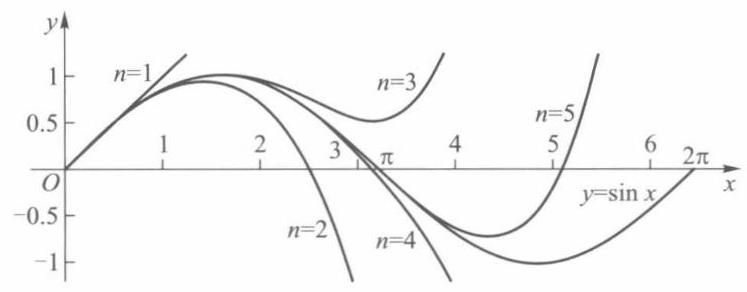
\includegraphics[width=.3\textwidth]{images/P103.jpg}
	\caption{图 $14-1$}
	\label{fig:P103}
\end{figure}
\[
x - \frac{{x}^{2}}{2} + \frac{{x}^{3}}{3} - \frac{{x}^{4}}{4} + \cdots  + {\left( -1\right) }^{n - 1}\frac{{x}^{n}}{n} + \cdots , \tag{5}
\]
用比式判别法容易求得级数 (5) 的收敛半径 \(R = 1\) ,且当 \(x = 1\) 时收敛,当 \(x =  - 1\) 时发散, 故级数 (5) 的收敛域是 \(( - 1,1\rbrack\) . 现在讨论在这收敛区间上它的余项的极限情形.

当 \(0 \leq  x \leq  1\) 时用拉格朗日型余项,有
\[
\left| {{R}_{n}\left( x\right) }\right|  = \left| {\frac{1}{\left( {n + 1}\right) !}{\left( -1\right) }^{n}\frac{n!}{{\left( 1 + \xi \right) }^{n + 1}}{x}^{n + 1}}\right|
\]
\[
= \left| {\frac{{\left( -1\right) }^{n}}{n + 1}{\left( \frac{x}{1 + \xi }\right) }^{n + 1}}\right|
\]
\[
\leq  \frac{1}{n + 1} \rightarrow  0\left( {n \rightarrow  \infty }\right) .
\]
对于 \(- 1 < x < 0\) 的情形,拉格朗日型余项不易估计,改用柯西型余项. 有
\[
\left| {{R}_{n}\left( x\right) }\right|  = \left| {\frac{1}{n!}{\left( -1\right) }^{n}\frac{n!}{{\left( 1 + \theta x\right) }^{n + 1}}{\left( 1 - \theta \right) }^{n}{x}^{n + 1}}\right|
\]
\[
= \frac{1}{1 + {\theta x}}{\left( \frac{1 - \theta }{1 + {\theta x}}\right) }^{n}{\left| x\right| }^{n + 1},\;0 \leq  \theta  \leq  1.
\]
因为 \(- 1 < x < 0\) ,故有 \(1 - \theta  \leq  1 + {\theta x}\) . 即 \(0 \leq  \frac{1 - \theta }{1 + {\theta x}} \leq  1\) ,所以
\[
\left| {{R}_{n}\left( x\right) }\right|  \leq  \frac{{\left| x\right| }^{n + 1}}{1 - \left| x\right| } \rightarrow  0\;\left( {n \rightarrow  \infty }\right) .
\]
这就证得在 \(( - 1,1\rbrack\) 上 \(\ln \left( {1 + x}\right)\) 等于其麦克劳林级数 (5).

将 (5) 式中 \(x\) 换成 \(x - 1\) 后就得到函数 \(f\left( x\right)  = \ln x\) 在 \(x = 1\) 处的泰勒展开式:
\[
\ln x = \left( {x - 1}\right)  - \frac{{\left( x - 1\right) }^{2}}{2} + \frac{{\left( x - 1\right) }^{3}}{3} + \cdots  + {\left( -1\right) }^{n - 1}\frac{{\left( x - 1\right) }^{n}}{n} + \cdots .
\]
它的收敛域为 \((0,2\rbrack\) .

%例 6
\begin{example}

\end{example}
讨论二项式函数 \(f\left( x\right)  = {\left( 1 + x\right) }^{\alpha }\) 的展开式.

当 \(\alpha\) 为正整数时,由二项式定理直接展开,就得到 \(f\) 的展开式,这已在前面例 2 中讨论过.

下面讨论 \(\alpha\) 不等于正整数时的情形,这时
\[
{f}^{\left( n\right) }\left( x\right)  = \alpha \left( {\alpha  - 1}\right) \cdots \left( {\alpha  - n + 1}\right) {\left( 1 + x\right) }^{\alpha  - n},\;n = 1,2,\cdots ,
\]
\[
{f}^{\left( n\right) }\left( 0\right)  = \alpha \left( {\alpha  - 1}\right) \cdots \left( {\alpha  - n + 1}\right) ,\;n = 1,2,\cdots .
\]
于是 \(f\left( x\right)\) 的麦克劳林级数是
\[
1 + {\alpha x} + \frac{\alpha \left( {\alpha  - 1}\right) }{2!}{x}^{2} + \cdots  + \frac{\alpha \left( {\alpha  - 1}\right) \cdots \left( {\alpha  - n + 1}\right) }{n!}{x}^{n} + \cdots . \tag{6}
\]
运用比式判别法,可得 (6) 的收敛半径 \(R = 1\) . 下面来证明 \(f\left( x\right)  = {\left( 1 + x\right) }^{\alpha }\) 的麦克劳林级数(6)在(-1,1)上收敛于 \({\left( 1 + x\right) }^{\alpha }\) . 这里同样可以用证明余项趋于零的方法来得到这个结论, 但我们希望给读者提供另一种处理类似问题的方法.

设级数 (6) 的和函数是 \(g\left( x\right)\) ,即
\[
g\left( x\right)  = 1 + {\alpha x} + \frac{\alpha \left( {\alpha  - 1}\right) }{2!}{x}^{2} + \cdots  + \frac{\alpha \left( {\alpha  - 1}\right) \cdots \left( {\alpha  - n + 1}\right) }{n!}{x}^{n} + \cdots ,x \in  \left( {-1,1}\right) .
\]
从 \(\left( {1 + x}\right) {\left( {\left( 1 + x\right) }^{\alpha }\right) }^{\prime } = \alpha {\left( 1 + x\right) }^{\alpha }\) 得到启发,对 \(g\left( x\right)\) 逐项求导,得
\[
{g}^{\prime }\left( x\right)  = \alpha \left\lbrack  {1 + \frac{\left( \alpha  - 1\right) }{1}x + \frac{\left( {\alpha  - 1}\right) \left( {\alpha  - 2}\right) }{2!}{x}^{2} + \cdots  + \frac{\left( {\alpha  - 1}\right) \cdots \left( {\alpha  - n + 1}\right) }{\left( {n - 1}\right) !}{x}^{n - 1} + \cdots }\right\rbrack  ,
\]
两边同乘 \(\left( {1 + x}\right)\) ,则右边 \({x}^{n}\) 项的系数为
\[
\frac{\left( {\alpha  - 1}\right) \cdots \left( {\alpha  - n + 1}\right) }{\left( {n - 1}\right) !} + \frac{\left( {\alpha  - 1}\right) \cdots \left( {\alpha  - n}\right) }{n!} = \frac{\left( {\alpha  - 1}\right) \cdots \left( {\alpha  - n + 1}\right) }{\left( {n - 1}\right) !}\left( {1 + \frac{\alpha  - n}{n}}\right)
\]
\[
= \frac{\alpha \left( {\alpha  - 1}\right) \cdots \left( {\alpha  - n + 1}\right) }{n!}\;\left( {n = 1,2,\cdots }\right) ,
\]
于是有
\[
\left( {1 + x}\right) {g}^{\prime }\left( x\right)  = {\alpha g}\left( x\right) ,x \in  \left( {-1,1}\right) .
\]
令
\[
F\left( x\right)  = \frac{g\left( x\right) }{{\left( 1 + x\right) }^{\alpha }},
\]
则 \(F\left( 0\right)  = g\left( 0\right)  = 1\) ,
\[
{F}^{\prime }\left( x\right)  = \frac{{\left( 1 + x\right) }^{\alpha }{g}^{\prime }\left( x\right)  - \alpha {\left( 1 + x\right) }^{\alpha  - 1}g\left( x\right) }{{\left( 1 + x\right) }^{2\alpha }} = \frac{\left( {1 + x}\right) {g}^{\prime }\left( x\right)  - {\alpha g}\left( x\right) }{{\left( 1 + x\right) }^{\alpha  + 1}} = 0.
\]
从而 \(F\left( x\right)  = F\left( 0\right)  = 1,x \in  \left( {-1,1}\right)\) ,即
\[
g\left( x\right)  = {\left( 1 + x\right) }^{\alpha },x \in  \left( {-1,1}\right) .
\]
所以在(-1,1)上,
\[
{\left( 1 + x\right) }^{\alpha } = 1 + {\alpha x} + \frac{\alpha \left( {\alpha  - 1}\right) }{2!}{x}^{2} + \cdots  + \frac{\alpha \left( {\alpha  - 1}\right) \cdots \left( {\alpha  - n + 1}\right) }{n!}{x}^{n} + \cdots . \tag{7}
\]
对于收敛区间端点的情形,它与 \(\alpha\) 的取值有关,其结果如下 (推导参见菲赫金哥尔茨著 《微积分学教程》第二卷第二分册):

当 \(\alpha  \leq   - 1\) 时,收敛域为(-1,1)；

当 \(- 1 < \alpha  < 0\) 时,收敛域为 \(( - 1,1\rbrack\) ;

当 \(\alpha  > 0\) 时,收敛域为 \(\left\lbrack  {-1,1}\right\rbrack\) .

当 (7) 式中 \(\alpha  =  - 1\) 时就得到
\[
\frac{1}{1 + x} = 1 - x + {x}^{2} + \cdots  + {\left( -1\right) }^{n}{x}^{n} + \cdots ,\;\left( {-1,1}\right) . \tag{8}
\]
当 \(\alpha  =  - \frac{1}{2}\) 时得到
\[
\frac{1}{\sqrt{1 + x}} = 1 - \frac{1}{2}x + \frac{1 \cdot  3}{2 \cdot  4}{x}^{2} - \frac{1 \cdot  3 \cdot  5}{2 \cdot  4 \cdot  6}{x}^{3} + \cdots ,\;( - 1,1\rbrack . \tag{9}
\]
一般地说, 只有少数比较简单的函数, 其幂级数展开式能直接从定义出发, 并根据定理 14.11 求得. 更多的情况是从已知的展开式出发, 通过变量代换、四则运算或逐项求导、逐项求积等方法, 间接地求得函数的幂级数展开式.

%例 7
\begin{example}

\end{example}
将 \({x}^{2}\) 与 \(- {x}^{2}\) 分别代入 (8) 式与 (9) 式,可得
\[
\frac{1}{1 + {x}^{2}} = 1 - {x}^{2} + {x}^{4} + \cdots  + {\left( -1\right) }^{n}{x}^{2n} + \cdots ,\;\left( {-1,1}\right) , \tag{10}
\]
\[
\frac{1}{\sqrt{1 - {x}^{2}}} = 1 + \frac{1}{2}{x}^{2} + \frac{1 \cdot  3}{2 \cdot  4}{x}^{4} + \frac{1 \cdot  3 \cdot  5}{2 \cdot  4 \cdot  6}{x}^{6} + \cdots ,\;\left( {-1,1}\right) . \tag{11}
\]
对于 (10) 式、(11) 式分别逐项求积可得函数 \(\arctan x\) 与 \(\arcsin x\) 的展开式:
\[
\arctan x = {\int }_{0}^{x}\frac{\mathrm{d}t}{1 + {t}^{2}}
\]
\[
= x - \frac{{x}^{3}}{3} + \frac{{x}^{5}}{5} + \cdots  + {\left( -1\right) }^{n}\frac{{x}^{{2n} + 1}}{{2n} + 1} + \cdots ,\;\left\lbrack  {-1,1}\right\rbrack  ,
\]
\[
\arcsin x = {\int }_{0}^{x}\frac{\mathrm{d}t}{\sqrt{1 - {t}^{2}}}
\]
\[
= x + \frac{1}{2}\frac{{x}^{3}}{3} + \frac{1 \cdot  3}{2 \cdot  4}\frac{{x}^{5}}{5} + \frac{1 \cdot  3 \cdot  5}{2 \cdot  4 \cdot  6}\frac{{x}^{7}}{7} + \cdots ,\;\left\lbrack  {-1,1}\right\rbrack  .
\]
由此可见, 熟悉某些初等函数的展开式, 对于一些函数的幂级数展开是极为方便的. 特别是前面介绍的例 3 至例 7 的结果, 对于用间接方法求幂级数展开式特别有用.

%例 8
\begin{example}

\end{example}
求函数 \(\left( {1 - x}\right) \ln \left( {1 - x}\right)\) 在 \(x = 0\) 处的幂级数展开式.

%解
\begin{solution}

\end{solution}
利用 \(\ln \left( {1 + x}\right)  = \mathop{\sum }\limits_{{n = 1}}^{\infty }{\left( -1\right) }^{n - 1}\frac{{x}^{n}}{n}\) ,得
\[
\left( {1 - x}\right) \ln \left( {1 - x}\right)  = \left( {1 - x}\right) \left( {-\mathop{\sum }\limits_{{n = 1}}^{\infty }\frac{{x}^{n}}{n}}\right)  =  - \mathop{\sum }\limits_{{n = 1}}^{\infty }\frac{{x}^{n}}{n} + \mathop{\sum }\limits_{{n = 1}}^{\infty }\frac{{x}^{n + 1}}{n}
\]
\[
=  - x - \mathop{\sum }\limits_{{n = 2}}^{\infty }\frac{{x}^{n}}{n} + \mathop{\sum }\limits_{{n = 2}}^{\infty }\frac{{x}^{n}}{n - 1}
\]
\[
=  - x + \mathop{\sum }\limits_{{n = 2}}^{\infty }\frac{{x}^{n}}{n\left( {n - 1}\right) },x \in  \left( {-1,1}\right) .
\]
\(\left( {1 - x}\right) \ln \left( {1 - x}\right)\) 在 \(x =  - 1\) 处连续,在 \(x = 1\) 处没有定义,而级数 \(\mathop{\sum }\limits_{{n = 2}}^{\infty }\frac{{x}^{n}}{n\left( {n - 1}\right) }\) 的收敛域为 \(\left\lbrack  {-1,1}\right\rbrack\) ,所以
\[
\left( {1 - x}\right) \ln \left( {1 - x}\right)  =  - x + \mathop{\sum }\limits_{{n = 2}}^{\infty }\frac{{x}^{n}}{n\left( {n - 1}\right) },\;x \in  \lbrack  - 1,1). \tag{0}
\]
%注
\begin{remark}

\end{remark}
上式右边的幂级数在 \(\left\lbrack  {-1,1}\right\rbrack\) 上都收敛,且在 \(x = 1\) 时收敛于 0,而(1 - x). \(\ln \left( {1 - x}\right)\) 只是它在 \(\lbrack  - 1,1)\) 上的和函数. 所以可以进一步写成
\[
- x + \mathop{\sum }\limits_{{n = 2}}^{\infty }\frac{{x}^{n}}{n\left( {n - 1}\right) } = \left\{  \begin{matrix} \left( {1 - x}\right) \ln \left( {1 - x}\right) , & x \in  \lbrack  - 1,1), \\  0, & x = 1. \end{matrix}\right.
\]
用类似的方法可得
\[
\ln \frac{1 + x}{1 - x} = 2\mathop{\sum }\limits_{{n = 0}}^{\infty }\frac{{x}^{{2n} + 1}}{{2n} + 1},\;x \in  \left( {-1,1}\right) . \tag{12}
\]
%例 9
\begin{example}

\end{example}
计算 \(\ln 2\) 的近似值,精确到 0.0001 .

%解
\begin{solution}

\end{solution}
可以在展开式 \(\ln \left( {1 + x}\right)  = \mathop{\sum }\limits_{{n = 1}}^{\infty }{\left( -1\right) }^{n - 1}\frac{{x}^{n}}{n}\) 中令 \(x = 1\) ,得 \(\ln 2 = \mathop{\sum }\limits_{{n = 1}}^{\infty }\frac{{\left( -1\right) }^{n - 1}}{n}\) , 这是一个交错级数, 需要计算 1 万项的和才能达到 0.0001 的精度, 收敛太慢! 为此在 ( 12 )式中令 \(\frac{1 + x}{1 - x} = 2\) ,即 \(x = \frac{1}{3}\) 代入 ( 12 )式,有
\[
\ln 2 = 2\left( {\frac{1}{3} + \frac{1}{3} \cdot  \frac{1}{{3}^{3}} + \cdots  + \frac{1}{{2n} + 1} \cdot  \frac{1}{{3}^{{2n} + 1}} + \cdots }\right) .
\]
估计余项如下:
\[
0 < {R}_{n} = 2\left( {\frac{1}{{2n} + 1} \cdot  \frac{1}{{3}^{{2n} + 1}} + \frac{1}{{2n} + 3} \cdot  \frac{1}{{3}^{{2n} + 3}} + \cdots }\right)
\]
\[
< \frac{2}{\left( {{2n} + 1}\right)  \cdot  {3}^{{2n} + 1}}\left( {1 + \frac{1}{{3}^{2}} + \frac{1}{{3}^{4}} + \cdots }\right)
\]
\[
= \frac{2}{\left( {{2n} + 1}\right)  \cdot  {3}^{{2n} + 1}} \cdot  \frac{1}{1 - \frac{1}{{3}^{2}}} = \frac{1}{4\left( {{2n} + 1}\right)  \cdot  {3}^{{2n} - 1}},
\]
取 \(n = 4\) ,就有 \(0 < {R}_{4} < \frac{1}{4 \cdot  9 \cdot  {3}^{7}} = \frac{1}{78732} < {0.0001}\) . 因此得到
\[
\ln 2 \approx  2\left( {\frac{1}{3} + \frac{1}{3} \cdot  \frac{1}{{3}^{3}} + \frac{1}{5} \cdot  \frac{1}{{3}^{5}} + \frac{1}{7} \cdot  \frac{1}{{3}^{7}}}\right)
\]
\[
\approx  2\left( {{0.33333} + {0.01235} + {0.00082} + {0.00007}}\right)
\]
\[
= {0.6931}\text{ . }
\]
作为本节的结束, 最后举例说明怎样用幂级数形式表示某些非初等函数. 在本章开头就已经提到幂级数的这种特有的功能.

%例 10
\begin{example}

\end{example}
用间接方法求非初等函数
\[
F\left( x\right)  = {\int }_{0}^{x}{\mathrm{e}}^{-{t}^{2}}\mathrm{\;d}t
\]
的幂级数展开式.

%解
\begin{solution}

\end{solution}
以 \(- {x}^{2}\) 代替例 3 中 \({\mathrm{e}}^{x}\) 展开式的 \(x\) ,得
\[
{\mathrm{e}}^{-{x}^{2}} = 1 - \frac{{x}^{2}}{1!} + \frac{{x}^{4}}{2!} - \frac{{x}^{6}}{3!} + \cdots  + \frac{{\left( -1\right) }^{n}{x}^{2n}}{n!} + \cdots ,
\]
\[
- \infty  < x <  + \infty \text{ . }
\]
再逐项求积就得到 \(F\left( x\right)\) 在 \(\left( {-\infty , + \infty }\right)\) 上的展开式
\[
F\left( x\right)  = {\int }_{0}^{x}{\mathrm{e}}^{-{t}^{2}}\mathrm{\;d}t
\]
\[
= x - \frac{1}{1!}\frac{{x}^{3}}{3} + \frac{1}{2!}\frac{{x}^{5}}{5} - \frac{1}{3!}\frac{{x}^{7}}{7} + \cdots  + \frac{{\left( -1\right) }^{n}}{n!}\frac{{x}^{{2n} + 1}}{{2n} + 1} + \cdots \text{ . }
\]
用上述级数的部分和逐项逼近 \(F\left( x\right)\) 的过程,如图 14-2 所示.

\begin{figure}
	\centering
	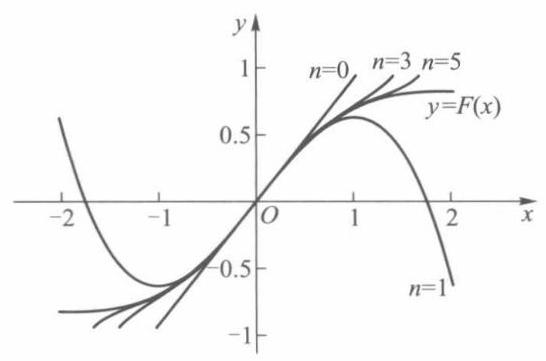
\includegraphics[width=.3\textwidth]{images/P104.jpg}
	\caption{图 $14-2$}
	\label{fig:P104}
\end{figure}

\subsection{习题 14.2}

1. 设函数 \(f\) 在区间(a, b)上的各阶导数一致有界,即存在正数 \(M\) ,对一切 \(x \in  \left( {a,b}\right)\) ,有
\[
\left| {{f}^{\left( n\right) }\left( x\right) }\right|  \leq  M,\;n = 1,2,\cdots .
\]
证明: 对(a, b)上任一点 \(x\) 与 \({x}_{0}\) 有
\[
f\left( x\right)  = \mathop{\sum }\limits_{{n = 0}}^{\infty }\frac{{f}^{\left( n\right) }\left( {x}_{0}\right) }{n!}{\left( x - {x}_{0}\right) }^{n}\;\left( {{f}^{\left( 0\right) }\left( x\right)  = f\left( x\right) ,0! = 1}\right) .
\]
2. 利用已知函数的幂级数展开式,求下列函数在 \(x = 0\) 处的幂级数展开式,并确定它收敛于该函数的区间:

(1) \({\mathrm{e}}^{{x}^{2}}\) ;

(2) \(\frac{{x}^{10}}{1 - x}\) ;

(3) \(\frac{x}{\sqrt{1 - {2x}}}\) ;

(4) \({\sin }^{2}x\) ;

(5) \(\frac{{\mathrm{e}}^{x}}{1 - x}\) ;

(6) \(\frac{x}{1 + x - 2{x}^{2}}\) ;

(7) \({\int }_{0}^{x}\frac{\sin t}{t}\mathrm{\;d}t\) ;

(8) \(\left( {1 + x}\right) {\mathrm{e}}^{-x}\) ;

(9) \(\ln \left( {x + \sqrt{1 + {x}^{2}}}\right)\) .

3. 求下列函数在 \(x = 1\) 处的泰勒展开式:

(1) \(f\left( x\right)  = 3 + {2x} - 4{x}^{2} + 7{x}^{3}\) ;

(2) \(f\left( x\right)  = \frac{1}{x}\) ;

(3) \(f\left( x\right)  = \sqrt{{x}^{3}}\) .

4. 求下列函数的麦克劳林级数展开式:

(1) \(\frac{x}{\left( {1 - x}\right) \left( {1 - {x}^{2}}\right) }\) ;

(2) \(x\arctan x - \ln \sqrt{1 + {x}^{2}}\) .

5. 试将 \(f\left( x\right)  = \ln x\) 按 \(\frac{x - 1}{x + 1}\) 的幂展开成幂级数.

\section{复变量的指数函数。欧拉公式}

先讲复数项级数. 设级数
\[
{u}_{1} + {u}_{2} + \cdots  + {u}_{n} + \cdots  \tag{1}
\]
中每一项都是复数 \({u}_{n} = {a}_{n} + \mathrm{i}{b}_{n}\;\left( {{a}_{n},{b}_{n}}\right.\) 为实数, \(\mathrm{i}\) 为虚部单位 \()\left( {n = 1,2,\cdots }\right)\) ,则 (1) 式可写成
\[
\left( {{a}_{1} + \mathrm{i}{b}_{1}}\right)  + \left( {{a}_{2} + \mathrm{i}{b}_{2}}\right)  + \cdots  + \left( {{a}_{n} + \mathrm{i}{b}_{n}}\right)  + \cdots . \tag{2}
\]
以 \({S}_{n}\) 表示 (2) 的第 \(n\) 个部分和,并记
\[
{R}_{n} = \mathop{\sum }\limits_{{k = 1}}^{n}{a}_{k},\;{I}_{n} = \mathop{\sum }\limits_{{k = 1}}^{n}{b}_{k},
\]
则有
\[
{S}_{n} = {R}_{n} + \mathrm{i}{I}_{n}.
\]
若 \(\mathop{\lim }\limits_{{n \rightarrow  \infty }}{R}_{n}\) 与 \(\mathop{\lim }\limits_{{n \rightarrow  \infty }}{I}_{n}\) 存在,则称级数 (1) 收敛,若用 \(A,B\) 分别表示这两个极限值,则级数 (1) 的和记为 \(A + \mathrm{i}B\) . 据此,级数 (1) 收敛的充要条件是: 级数
\[
\mathop{\sum }\limits_{{n = 1}}^{\infty }{a}_{n}\;\text{ 与 }\;\mathop{\sum }\limits_{{n = 1}}^{\infty }{b}_{n}
\]
都收敛.

级数 (1) 各项 \({u}_{n}\) 的模为
\[
\left| {u}_{n}\right|  = \sqrt{{a}_{n}^{2} + {b}_{n}^{2}},\;n = 1,2,\cdots .
\]
若级数
\[
\left| {u}_{1}\right|  + \left| {u}_{2}\right|  + \cdots  + \left| {u}_{n}\right|  + \cdots
\]
收敛, 则称级数 (1) 绝对收敛. 由关系式
\[
\left| {a}_{n}\right|  \leq  \left| {u}_{n}\right| ,\;\left| {b}_{n}\right|  \leq  \left| {u}_{n}\right| ,\;n = 1,2,\cdots
\]
可证得: 若级数 (1) 绝对收敛, 则级数 (1) 必收敛.

设 \({c}_{n}\left( {n = 0,1,2,\cdots }\right)\) 为复数, \(z\) 为复变量,则称级数
\[
{c}_{0} + {c}_{1}z + {c}_{2}{z}^{2} + \cdots  + {c}_{n}{z}^{n} + \cdots  \tag{3}
\]
为复数项幂级数. 若在 \(z = {z}_{0}\) 处级数 (3) 收敛,则称它在点 \({z}_{0}\) 收敛. 所有使级数 (3) 收敛的全体复数构成复数项幂级数 (3) 的收敛域. 记
\[
\rho  = \mathop{\lim }\limits_{{n \rightarrow  \infty }}\sqrt[n]{\left| {c}_{n}\right| },
\]
这时和 §1 实数项幂级数一样可证明: 级数 (3) 对一切满足 \(\left| z\right|  < \frac{1}{\rho }\) 的 \(z\) 不仅收敛,而且绝对收敛; 对一切 \(\left| z\right|  > \frac{1}{\rho }\) 的 \(z\) ,级数 (3) 是发散的. 现以 \(R = \frac{1}{\rho }\) 表示复数项幂级数 (3) 的收敛半径 (当 \(\rho  = 0\) 时, \(R =\)  \(+ \infty\) ; 当 \(\rho  =  + \infty\) 时, \(R = 0\) ),则级数 (3) 的收敛范围是复平面上的以原点为中心, \(R\) 为半径的圆.

例如级数
\[
1 + z + \frac{{z}^{2}}{2!} + \cdots  + \frac{{z}^{n}}{n!} + \cdots , \tag{4}
\]
由于
\[
\mathop{\lim }\limits_{{n \rightarrow  \infty }}\sqrt[n]{\left| {c}_{n}\right| } = \mathop{\lim }\limits_{{n \rightarrow  \infty }}\sqrt[n]{\frac{1}{n!}} = 0,
\]
故级数 (4) 的收敛半径 \(R =  + \infty\) ,即 (4) 在整个复平面上都是收敛的,当 \(z\) 为实变量 \(x\) 时,(4) 的和函数为实变量的指数函数 \({\mathrm{e}}^{x}\) . 因此,我们也把级数 (4) 的和函数定义为复变量 \(z\) 的指数函数 \({\mathrm{e}}^{z}\) ,即
\[
{\mathrm{e}}^{z} = 1 + z + \frac{{z}^{2}}{2!} + \cdots  + \frac{{z}^{n}}{n!} + \cdots . \tag{5}
\]
用同样的方法可定义复变量的正弦函数与余弦函数:
\[
\sin z = z - \frac{{z}^{3}}{3!} + \frac{{z}^{5}}{5!} + \cdots  + {\left( -1\right) }^{n - 1}\frac{{z}^{{2n} - 1}}{\left( {{2n} - 1}\right) !} + \cdots , \tag{6}
\]
\[
\cos z = 1 - \frac{{z}^{2}}{2!} + \frac{{z}^{4}}{4!} + \cdots  + {\left( -1\right) }^{n}\frac{{z}^{2n}}{\left( {2n}\right) !} + \cdots . \tag{7}
\]
它们的收敛域都是整个复平面.

以 \(\mathrm{i}z\) 代替 (5) 式中的 \(z\) ,可得
\[
{\mathrm{e}}^{\mathrm{i}z} = 1 + \mathrm{i}z + \frac{{\left( \mathrm{i}z\right) }^{2}}{2!} + \cdots  + \frac{{\left( \mathrm{i}z\right) }^{n}}{n!} + \cdots
\]
\[
= 1 + \mathrm{i}z - \frac{{z}^{2}}{2!} - \mathrm{i}\frac{{z}^{3}}{3!} + \frac{{z}^{4}}{4!} + \mathrm{i}\frac{{z}^{5}}{5!} + \cdots
\]
\[
= \left( {1 - \frac{{z}^{2}}{2!} + \frac{{z}^{4}}{4!} + \cdots }\right)  + \mathrm{i}\left( {z - \frac{{z}^{3}}{3!} + \frac{{z}^{5}}{5!} + \cdots }\right) .
\]
联系 (6) 式与 (7) 式, 就有
\[
{\mathrm{e}}^{\mathrm{i}z} = \cos z + \mathrm{i}\sin z.
\]
当 \(z\) 为实变量 \(x\) 时,则得
\[
{\mathrm{e}}^{\mathrm{i}x} = \cos x + \mathrm{i}\sin x, - \infty  < x <  + \infty .
\]
它称为欧拉公式. 这个公式给出了 (实变量) 指数函数与三角函数之间的关系.

由于任一复数 \(z\) 都可写作 \(r\left( {\cos \theta  + \mathrm{i}\sin \theta }\right)\) ( \(r\) 为 \(z\) 的模,即 \(\left| z\right|  = r,\theta  = \arg z\) 为 \(z\) 的辐角),那么由欧拉公式可得复数的指数形式
\[
z = r\left( {\cos \theta  + \mathrm{i}\sin \theta }\right)  = r{\mathrm{e}}^{\mathrm{i}\theta }.
\]
与实幂级数一样, 由级数的乘法运算可得
\[
{\mathrm{e}}^{{z}_{1} + {z}_{2}} = {\mathrm{e}}^{{z}_{1}}{\mathrm{e}}^{{z}_{2}}.
\]
将 \(z = x + \mathrm{i}y\) 代入上式,则有
\[
{\mathrm{e}}^{z} = {\mathrm{e}}^{x + \mathrm{i}y} = {\mathrm{e}}^{x}{\mathrm{e}}^{\mathrm{i}y} = {\mathrm{e}}^{x}\left( {\cos y + \mathrm{i}\sin y}\right) .
\]
\subsection{习题 14.3}

1. 证明棣莫弗 (de Moivre) 公式
\[
\cos {nx} + \mathrm{i}\sin {nx} = {\left( \cos x + \mathrm{i}\sin x\right) }^{n}.
\]
2. 应用欧拉公式与棣莫弗公式证明:

(1) \({\mathrm{e}}^{x\cos \alpha }\cos \left( {x\sin \alpha }\right)  = \mathop{\sum }\limits_{{n = 0}}^{\infty }\frac{{x}^{n}}{n!}\cos {n\alpha }\) ;

(2) \({\mathrm{e}}^{x\cos \alpha }\sin \left( {x\sin \alpha }\right)  = \mathop{\sum }\limits_{{n = 0}}^{\infty }\frac{{x}^{n}}{n!}\sin {n\alpha }\) .

\section{总练习题}

1. 证明: 当 \(\left| x\right|  < \frac{1}{2}\) 时,
\[
\frac{1}{1 - {3x} + 2{x}^{2}} = 1 + {3x} + 7{x}^{2} + \cdots  + \left( {{2}^{n} - 1}\right) {x}^{n - 1} + \cdots .
\]

2. 求下列函数的幂级数展开式:

(1) \(f\left( x\right)  = \left( {1 + x}\right) \ln \left( {1 + x}\right)\) ;

(2) \(f\left( x\right)  = {\sin }^{3}x\) ;

(3) \(f\left( x\right)  = {\int }_{0}^{x}\cos {t}^{2}\mathrm{\;d}t\) .

3. 确定下列幂级数的收敛域, 并求其和函数:

(1) \(\mathop{\sum }\limits_{{n = 1}}^{\infty }{n}^{2}{x}^{n - 1}\) ;

(2) \(\mathop{\sum }\limits_{{n = 0}}^{\infty }\frac{{2n} + 1}{{2}^{n + 1}}{x}^{2n}\) ;

(3) \(\mathop{\sum }\limits_{{n = 1}}^{\infty }n{\left( x - 1\right) }^{n - 1}\) ;

(4) \(\mathop{\sum }\limits_{{n = 1}}^{\infty }{\left( -1\right) }^{n - 1}\frac{{x}^{{2n} + 1}}{{\left( 2n\right) }^{2} - 1}\) .

4. 应用幂级数性质求下列级数的和:

(1) \(\mathop{\sum }\limits_{{n = 1}}^{\infty }\frac{n}{\left( {n + 1}\right) !}\) ;

(2) \(\mathop{\sum }\limits_{{n = 0}}^{\infty }\frac{{\left( -1\right) }^{n}}{{3n} + 1}\) .

5. 设函数
\[
f\left( x\right)  = \mathop{\sum }\limits_{{n = 1}}^{\infty }\frac{{x}^{n}}{{n}^{2}}
\]
定义在 \(\left\lbrack  {0,1}\right\rbrack\) 上,证明它在(0,1)上满足下述方程:
\[
f\left( x\right)  + f\left( {1 - x}\right)  + \ln x\ln \left( {1 - x}\right)  = f\left( 1\right) .
\]
6. 利用函数的幂级数展开式求下列不定式极限:

(1) \(\mathop{\lim }\limits_{{x \rightarrow  \infty }}\left\lbrack  {x - {x}^{2}\ln \left( {1 + \frac{1}{x}}\right) }\right\rbrack\) ;

(2) \(\mathop{\lim }\limits_{{x \rightarrow  0}}\frac{x - \arcsin x}{{\sin }^{3}x}\) .

